\section{Wrong conjectures}

These is a collection of wrong ``proofs'' and conjectures:

\begin{conjecture}
  Let $T$ be an intree. Let $z_1, z_2$ be two new tasks that will be added to this intree with $level(z_1) > level(z_2)$. Then, $T^*\left(T\cup\left\{ z_1 \right\}\right) > T^*\left( T\cup\left\{ z_2 \right\} \right)$.
\end{conjecture}

\begin{lemma}
  \label{lem:p3-adding-tasks-level-keep-scheduled-same-inequality}
  Let $I$ be an intree and $x, y$ ready tasks within this intree (it may be the case that $x=y$ if there is only one ready task or if adding new tasks as described below requires this). Let $z_1, z_2$ be two new tasks that will be added to this intree with $level(z_1) > level(z_2)$. The tasks $z_1$ and $z_2$ shall be added in such a way that neither $x$ nor $y$ is a successor of $z_1$ resp. $z_2$ (i.e. $x,y$ stay ready). 
  
  By $T^*_{t_1,t_2,t_3}(I)$ we denote the optimal expected run time that can be acchieved if we \emph{initially} schedule all tasks from the set $\left\{ t_1,t_2,t_3 \right\}$.
  
  Then, if $x,y$ and $z_1$ resp. $z_2$ are used as initial tasks, we have the following for the best acchievable expected run times (for respective initial tasks):
  \begin{equation}
    \label{eq:lemma-p3-adding-tasks-level-keep-scheduled-same-inequality}
    T^{*}_{x,y,z_1}\left(I\cup\left\{ z_1 \right\}\right) > T^{*}_{x,y,z_2}\left( I\cup\left\{ z_2 \right\} \right)
  \end{equation}
\end{lemma}

\todo{Counterexample is 001235677, where we add tasks on node 4 resp. node 5. Problem is -- again -- in the induction step!}

\begin{proof}
  We prove the claim by induction on the number of nodes:
  
  The induction basis is the case where we have intrees with 3 tasks\footnote{We start by 3 tasks since these trees are the only ones that allow adding $z_1$ and $z_2$ at different levels such that both $x$ and $y$ stay ready. For an intree with two tasks, the claim can be seen by simply examining that $T(0,0)<T(0,1)$\todo{Improve this footnote.}.} (all of them are depicted in figure \ref{fig:p3-lemma-adding-intrees-induction-start} (only the black nodes)).
  
  \begin{figure}[t]
    \centering
    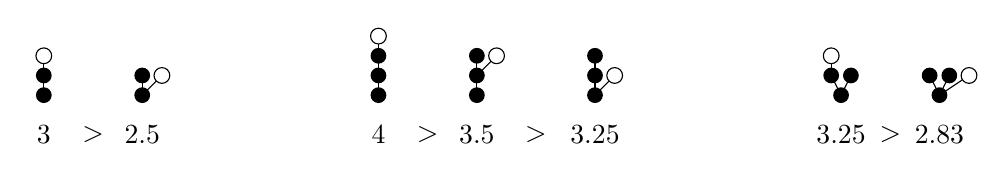
\begin{tikzpicture}[scale=0.25]
      \newcommand{\treeone}{
        \fill(0,0) circle (0.4);
        \fill(0,1) circle (0.4);
        \fill(0,2) circle (0.4);
        \draw(0,0) -- (0,1);
        \draw(0,1) -- (0,2);
      }
      \newcommand{\treetwo}{
        \fill(0,0) circle (0.4);
        \fill(-.50,1) circle (0.4);
        \fill(.50,1) circle (0.4);
        \draw(0,0) -- (0.5,1);
        \draw(0,0) -- (-.5,1);
      }
      \newcommand{\treethree}{
        \fill(0,0) circle (0.4);
        \fill(0,1) circle (0.4);
        \draw(0,0) -- (0,1);
      }
      % \begin{scope}
      %   \treeone;
      % \end{scope}
      % \begin{scope}[xshift=9cm]
      %   \treetwo;
      % \end{scope}

      \begin{scope}[yshift=-5cm, xshift=-20.5cm]
        \begin{scope}
          \treethree;
          \draw(0,1) -- (0,2);
          \draw[fill=white](0,2) circle (0.4);
          \node at (0,-2) {3};
        \end{scope}
        \node at (2.5,-2) {$>$};
        \begin{scope}[xshift=5cm]
          \treethree;
          \draw(0,0) -- (1,1);
          \draw[fill=white](1,1) circle (0.4);
          \node at (0,-2) {2.5};
        \end{scope}
      \end{scope}

      \begin{scope}[yshift=-5cm, xshift=-3.5cm]
        \begin{scope}
          \treeone;
          \draw(0,2) -- (0,3);
          \draw[fill=white](0,3) circle (0.4);
          \node at (0,-2) {4};
        \end{scope}
        \node at (2.5,-2) {$>$};
        \begin{scope}[xshift=5cm]
          \treeone;
          \draw(0,1) -- (1,2);
          \draw[fill=white](1,2) circle (0.4);
          \node at (0,-2) {3.5};
        \end{scope}
        \node at (8,-2) {$>$};
        \begin{scope}[xshift=11cm]
          \treeone;
          \draw(0,0) -- (1,1);
          \draw[fill=white](1,1) circle (0.4);
          \node at (0,-2) {3.25};
        \end{scope}
        % \node at (4,-1.5) {$4 > 3.5 > 3.25$};
      \end{scope}

      \begin{scope}[yshift=-5cm, xshift=20cm]
        \begin{scope}[xshift=0cm]
          \treetwo;
          \draw(-.5,1) -- (-.5,2);
          \draw[fill=white](-.5,2) circle (0.4);
          \node at (0,-2) {3.25};
        \end{scope}
        \node at (2.5,-2) {$>$};
        \begin{scope}[xshift=5cm]
          \treetwo;
          \draw(0,0) -- (1.5,1);
          \draw[fill=white](1.5,1) circle (0.4);
          \node at (0,-2) {2.83};
        \end{scope}
      \end{scope}
      
    \end{tikzpicture}
    \caption{Adding new tasks to intrees with less than four nodes. The original (2- resp. 3-node) intrees are drawn black, the newly added tasks are drawn white. Below each intree, we see the corresponding optimal expected run time. The lower the level of the newly added task, the lower the expected run time. This serves as basis for the induction proof for lemma \ref{lem:p3-adding-tasks-level-keep-scheduled-same-inequality}.}
    \label{fig:p3-lemma-adding-intrees-induction-start}
  \end{figure}

  If we add two tasks $z_1$ and $z_2$ with $level(z_1)>level(z_2)$ in a way such that the original ready tasks stay ready, we obtain the intrees depicted in figure \ref{fig:p3-lemma-adding-intrees-induction-start} (trees \emph{including} the white nodes). By simply computing the expected optimal run times, we can confirm our claim for intrees with 3 nodes.

  We now do the induction step by considering an intree with $n$ tasks. Let $x,y$ be ready tasks and $z_1$ and $z_2$ to be added with $level(z_1) > level(z_2)$. We can now compare the two runs that can occur if $x,y,z_1$ resp. $x,y,z_2$ are initially scheduled. 
  Therefore, we consider what happens in $I_1$ resp. $I_2$ if either $x$, $y$ or $z_1/z_2$ finishes first:

  \begin{itemize}
  \item If $z_1$ resp. $z_2$ is the first task to finish, the resulting intree is exactly $I$ as initially defined. Thus, the remaining run times for these cases are identical. We denote the task that may be chosen additionally\footnote{It may be the case that only $x$ and $y$ can be scheduled. In this case, we simply assume $z'=x$ to simplify notation.} to $x$ and $y$ by $z'$. The corresponding run time for the resulting intree is then $T^*_{x,y,z'}$
  \item If $x$ is the first task to finish, then the resulting intrees are $I_{1,x}'=I_1\setminus\left\{ x \right\}$ resp. $I_{2,x}'=I_2\setminus\left\{ x \right\}$. Denote by $x'$ the following:
    \begin{equation*}
      x' =
      \begin{cases}
        \text{successor of } x, & \text{if $x$ was the only predecessor of its successor} \\
        y, & \text{otherwise}
      \end{cases}
    \end{equation*}
    
    This, basically, simplifies notation a bit.
    
    The intrees $I_{1,x}'$ and $I_{2,x}'$ have exactly $n$ tasks -- and they have a common subtree, namely $I''_x=I_{1,x}'\setminus\left\{ z_1 \right\}=I_{2,x}'\setminus\left\{ z_2 \right\}$.
    
    We can now apply the induction hypothesis for the intree $I''_x$, since this intree contains only $n-1$ tasks: We have an intree with $n-1$ tasks (namely $I''_x$) and two tasks $z_1$ and $z_2$ with $level(z_1)>level(z_2)$, which means that $T^*_{x',y,z_1}(I'_{1,x})>T^*_{x',y,z_2}(I'_{2,x})$.
  \item If $y$ is the first task to finish, we argue similar to the $x$ case, thereby considering $I'_{1,y},I'_{2,y}$ and $I''_y$ which are all defined analogously. This finally yields the following inequality: $T^*_{x,y',z_1}(I'_{1,y}) > T^*_{x,y',z_2}(I'_{2,y})$.
  \end{itemize}

  The above considerations are illustrated in figure \ref{fig:p3-adding-tasks-level-keep-scheduled-same-inequality}.
  
  \begin{figure}[t]
    \centering
    \newcommand{\drawx}{
      \node[draw=black,circle] at (.9,3) {$x$};
    }
    \newcommand{\drawxx}{
      \node[draw=black,circle] at (.7,2) {$x'$};
    }
    \newcommand{\drawy}{
      \node[draw=black,circle] at (-1.5,4) {$y$};
    }
    \newcommand{\drawyy}{
      \node[draw=black,circle] at (-1.5,3) {$y'$};
    }
    \newcommand{\rawtriangle}{
      \draw
      [dotted, very thick,
      %fill=white!90!black, 
      rounded corners]
      (0,0) -- (3,2) -- (3.5,8) -- (-3.5,8) -- (-3,2) -- cycle;
    }
    \newcommand{\treetriangle}{
      \rawtriangle;
      \drawx;
      \drawy;
    }
    \newcommand{\abstand}{7.5cm}
    \begin{tikzpicture}[scale=.4]
      \begin{scope}[xshift=-\abstand]
        \treetriangle
        \node[draw=black,circle] at (0,6.5) {$z_1$};
      \end{scope}
      \begin{scope}[xshift=\abstand]
        \treetriangle
        \node[draw=black,circle] at (1,5) {$z_2$};
      \end{scope}
      
      \begin{scope}[xshift=-2*\abstand, yshift=-9cm]
        \rawtriangle
        \node[draw=black,circle] at (0,6.5) {$z_1$};
        \drawxx;
        \drawy;
      \end{scope}

      \begin{scope}[xshift=-\abstand, yshift=-9cm]
        \rawtriangle
        \node[draw=black,circle] at (0,6.5) {$z_1$};
        \drawx;
        \drawyy;
      \end{scope}

      \begin{scope}[xshift=0, yshift=-9cm]
        \treetriangle
        \node[draw=black,circle] at (.3,5.5) {$z'$};
      \end{scope}
      
      \begin{scope}[xshift=\abstand, yshift=-9cm]
        \rawtriangle
        \node[draw=black,circle] at (1,5) {$z_2$};
        \drawxx;
        \drawy;
      \end{scope}

      \begin{scope}[xshift=2*\abstand, yshift=-9cm]
        \rawtriangle
        \node[draw=black,circle] at (1,5) {$z_2$};
        \drawx;
        \drawyy;
      \end{scope}
      
      \draw[thick,->](-\abstand,0) -- +(0,-.8);
      \draw[thick,->](-\abstand-2cm,1) -- +(-\abstand+4cm,-1.6);
      \draw[thick,->](-\abstand+2cm,1) -- +(\abstand-4cm,-1.6);

      \begin{scope}[xshift=2*\abstand]
        \draw[thick,->](-\abstand,0) -- +(0,-.8);
        \draw[thick,->](-\abstand-2cm,1) -- +(-\abstand+4cm,-1.6);
        \draw[thick,->](-\abstand+2cm,1) -- +(\abstand-4cm,-1.6);
      \end{scope}
      
      % legend      
      \draw[decoration=brace,decorate=true](-11,8.25) --node[above]{$I_1$} +(7,0);
      \draw[decoration=brace,decorate=true](  4,8.25) --node[above]{$I_2$} +(7,0);
      \draw[decoration={brace,mirror},decorate=true](  -18,-9.5) --node[below, yshift=-.2cm]{$I'_{1,x}$} +(6,0);
      \draw[decoration={brace,mirror},decorate=true](-10.5,-9.5) --node[below, yshift=-.2cm]{$I'_{1,y}I$} +(6,0);
      \draw[decoration={brace,mirror},decorate=true](   -3,-9.5) --node[below, yshift=-.2cm]{$I$} +(6,0);
      \draw[decoration={brace,mirror},decorate=true](  4.5,-9.5) --node[below, yshift=-.2cm]{$I'_{2,x}$} +(6,0);
      \draw[decoration={brace,mirror},decorate=true](   12,-9.5) --node[below, yshift=-.2cm]{$I'_{2,y}$} +(6,0);
    \end{tikzpicture}

    \caption{Proof sketch for lemma \ref{lem:p3-adding-tasks-level-keep-scheduled-same-inequality}. By induction hypothesis, we have that $T^*_{x',y,z_1}(I'_{1,x}) > T^*_{x',y,z_2}(I'_{2,x})$ and $T^*_{x,y',z_1}(I'_{1,y}) > T^*_{x,y',z_2}(I'_{2,y})$, from which we deduce $T^*_{x,y,z_1}(I_1) > T^*_{x,y,z_2}(I_2)$.}
    \label{fig:p3-adding-tasks-level-keep-scheduled-same-inequality}
  \end{figure}
  
  Now we argue that the run times for $I_1$ and $I_2$ can be computed as follows:
  \begin{align*}
    T^*_{x,y,z_1}(I_1) & = 
      \frac{1}{3} + 
      \frac{1}{3}\cdot \left( 
        T_{x,y,z'}^*(I) + 
        T^*_{x',y,z_1}(I'_{1,x}) +
        T^*_{x,y',z_1}(I'_{1,y}) 
      \right)
      \\
    T^*_{x,y,z_2}(I_2) & = 
      \frac{1}{3} + 
      \frac{1}{3}\cdot \left( 
        T_{x,y,z'}^*(I) + 
        T^*_{x',y,z_2}(I'_{2,x}) +
        T^*_{x,y',z_2}(I'_{2,y}) 
      \right)
  \end{align*}

  We will now use the aforementioned inequalities $T^*_{x',y,z_1}(I'_{1,x}) > T^*_{x',y,z_2}(I'_{2,x})$ and $T^*_{x,y',z_1}(I'_{1,y}) > T^*_{x,y',z_2}(I'_{2,y})$. Which gives us that
\begin{align*}
    T^*_{x,y,z_1}(I_1) & = 
      \frac{1}{3} + 
      \frac{1}{3}\cdot \left( 
        T_{x,y,z'}^*(I) + 
        T^*_{x',y,z_1}(I'_{1,x}) +
        T^*_{x,y',z_1}(I'_{1,y}) 
      \right)
      > 
      \\
      & >
      \frac{1}{3} + 
      \frac{1}{3}\cdot \left( 
        T_{x,y,z'}^*(I) + 
        T^*_{x',y,z_2}(I'_{2,x}) +
        T^*_{x,y',z_2}(I'_{2,y}) 
      \right) 
      = T^*_{x,y,z_2}(I_2).
  \end{align*}

  This proves our claim.    
\end{proof}

%%% Local Variables:
%%% TeX-master: "../thesis.tex"
%%% End: 